% Appendix B
 
\chapter{Designing Figures}

This section contains recommendations on designing effective figures. We will cover graphs as well as diagrams.

We compiled the material in this appendix from the following sources:
\begin{itemize}
  \item the book ``Designing Science Presentations: A Visual Guide to Figures, Papers, Slides, Posters, and More'' \cite{Carter12},
  \item the book ``Information Visualization: Perception for Design'' \cite{Ware12}, and 
  \item …
\end{itemize}

\section{Fundamental Concepts}

\subsection{Gestalt Theory}

% Gestalt Theory and Instructional Design , Moore and Fitz 1993
% http://citeseerx.ist.psu.edu/viewdoc/download?doi=10.1.1.1026.6390&rep=rep1&type=pdf
% Gestalt

% alignment
% proximity
% connectedness
% 

\subsection{Color}

You are probably used to defining colors in terms of red, green, and blue (RGB) or cyan, magenta, yellow, and black (CMYK). A third way, which is more useful, is the \textbf{HSB model}. It defines color in terms of hue, saturation, and brightness.\sidenote{Read the primer at \url{https://learnui.design/blog/the-hsb-color-system-practicioners-primer.html} for more details.} Consider the color picker shown in Fig.~\ref{fig:hsb} for an example.

\begin{figure}
\centering
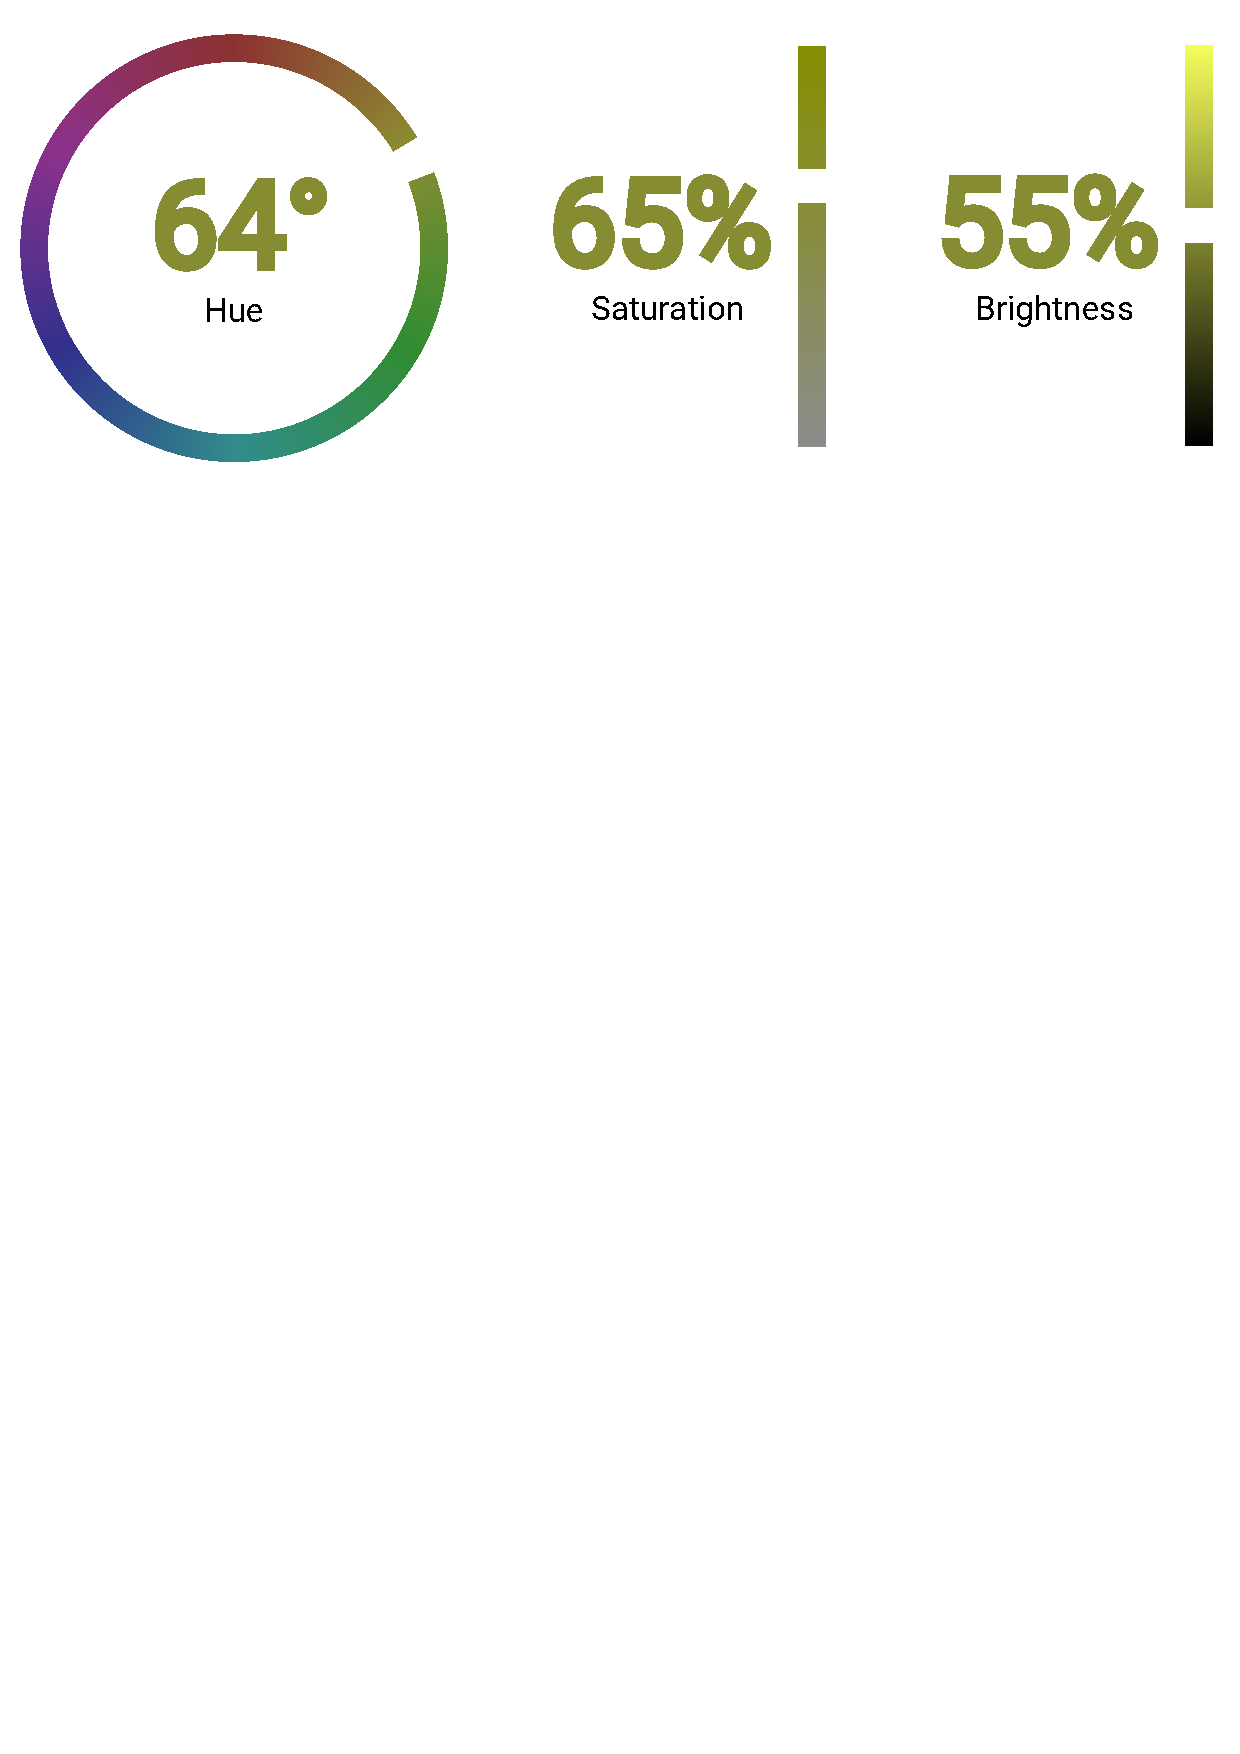
\includegraphics[width=0.85\textwidth]{color-hsb}
\sidecaption{\label{fig:hsb} A HSB color picker (\url{https://codepen.io/HunorMarton/full/eWvewo})}[-1\baselineskip]
\end{figure}

The first value, \textbf{hue}, defines the color according to its position (given in degrees ranging from 0 to 360) on the color wheel. For instance, the value 60 corresponds to the hue yellow. \textbf{Saturation} (0 to 100) corresponds to the richness of the color, where 0 means that there is no trace of the hue, i.\,e., a gray color between white and black. The value 100 means that the hue is fully present, i.\,e., the color is as colorful as possible. The final value is \textbf{brightness} (0 to 100). A value of 0 corresponds to a solid black (regardless of hue and saturation), a value of 100 corresponds to the brightest version of the hue at the given saturation.

Different colors are often used to ease visual perception (cf. Fig.~\ref{fig:coloredgraphs}). For instance, it can be used for emphasis, to group subsets of elements, or to make it easier to distinguish different elements that have a similar shape.

\begin{marginfigure}
\centering
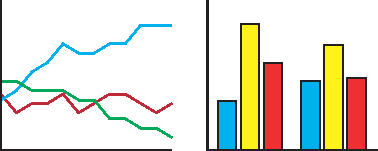
\includegraphics[width=1\textwidth]{color-plots}
\caption{\label{fig:coloredgraphs} Using colors to ease visual perception \cite{Carter12}.}%[-1\baselineskip]
\end{marginfigure}


Be aware of the monochrome representation of colors, which makes it impossible to distinguish a subset of colors. Red and green are particularly difficult to distinguish in monochrome print, especially if they have the same saturation and brightness (cf. Fig.~\ref{fig:monochrome}).

\begin{marginfigure}
\centering
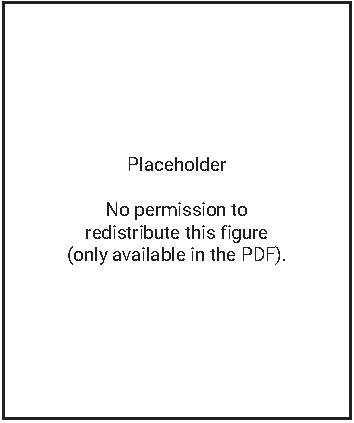
\includegraphics[width=0.8\textwidth]{color-mono}
\caption{\label{fig:monochrome} Colors in monochrome \cite{Carter12}.}%[-1\baselineskip]
\end{marginfigure}

The risk of confusion in monochrome prints is not the only reason why changing the hue is problematic. Different hues are difficult to make out when the area is small, as in the line plot in  Fig.~\ref{fig:coloredgraphs}. Moreover, different colors (hues) have different connotations (such as green means good, red means danger). Finally, different colors have different visual weight that may create unwanted emphasis (blue is heavier than orange).

Therefore, it is often better to stick with one hue and use different levels of brightness or saturation to ease visual perception. Figure~\ref{fig:monographs} uses three shades of gray and is easier to read than the colorful version in Fig.~\ref{fig:coloredgraphs}.


\begin{marginfigure}
\centering
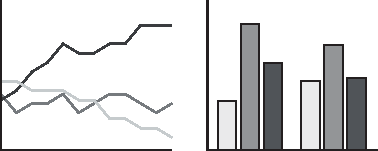
\includegraphics[width=1\textwidth]{color-plots-mono}
\caption{\label{fig:monographs} Shades of gray can be very effective \cite{Carter12}.}%[-1\baselineskip]
\end{marginfigure}

When you use more than four different grayscale colors, however, the differences become too small to perceive with ease. Too many grayscale colors are especially problematic when color is used on its own, such as in line plots. It is less problematic in bar plots, because the bars can be sorted with decreasing levels of brightness to create (good) redundancy. If brightness is used to encode values of data, darker color should be used for higher values.

Similar principles apply for saturation: ``If using color saturation to encode numerical quantity, use greater saturation to represent greater numerical quantities. Avoid using a saturation sequence to encode more than three values.'' \cite{Ware12} Consider varying both brightness and saturation at the same time to create shades that are easier to distinguish from another.

The effects of different levels of saturation vary depending on the size of the colored area (cf. Fig.~\ref{fig:saturation}). If you consider varying saturation, stick to the following guidelines: ``Use more saturated colors when color coding small symbols, thin lines, or other small areas. Use less saturated colors for coding large areas.'' \cite{Ware12}

\begin{marginfigure}
\centering
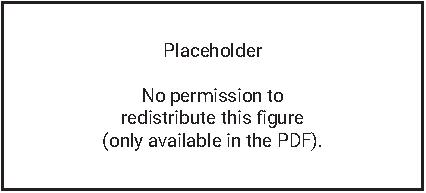
\includegraphics[width=1\textwidth]{color-saturation}
\caption{\label{fig:saturation} Use less saturation for large shapes, and more for thin lines \cite{Ware12}.}%[-2\baselineskip]
\end{marginfigure}



\section{Diagrams}

You can use diagrams to describe concepts and their relationship, the structure of systems, interactions, and (experimental) procedures.

\subsection{Common Problems}

% infohq

% examples

\subsection{Before You Start}

Questions to ask when designing a diagram as proposed by \cite{Carter12}.
\begin{itemize}
\item What is absolutely necessary to show?
\item What is not necessary to show?
\item What is most important and should be emphasized?
\item What is not important and should be secondary to the main message?
\item What are the relationships between individual elements?
\item Does the diagram require a precise depiction of time?
\item Does the diagram require a precise depiction of distance?
\item What symbols should be consistent throughout the diagram?
\end{itemize}


\subsection{Emphasizing Elements}

Good diagrams are self-explanatory and guide the reader's attention. Humans constantly search for patterns and deviations. Consistent use of shapes and colors indicates that the presented elements are similar (cf. Fig.~\ref{fig:emphasis}). Deviation from the norm indicate differences that need attention. Be aware of that and do not create emphasis unintentionally.

\begin{figure}[t]
\centering
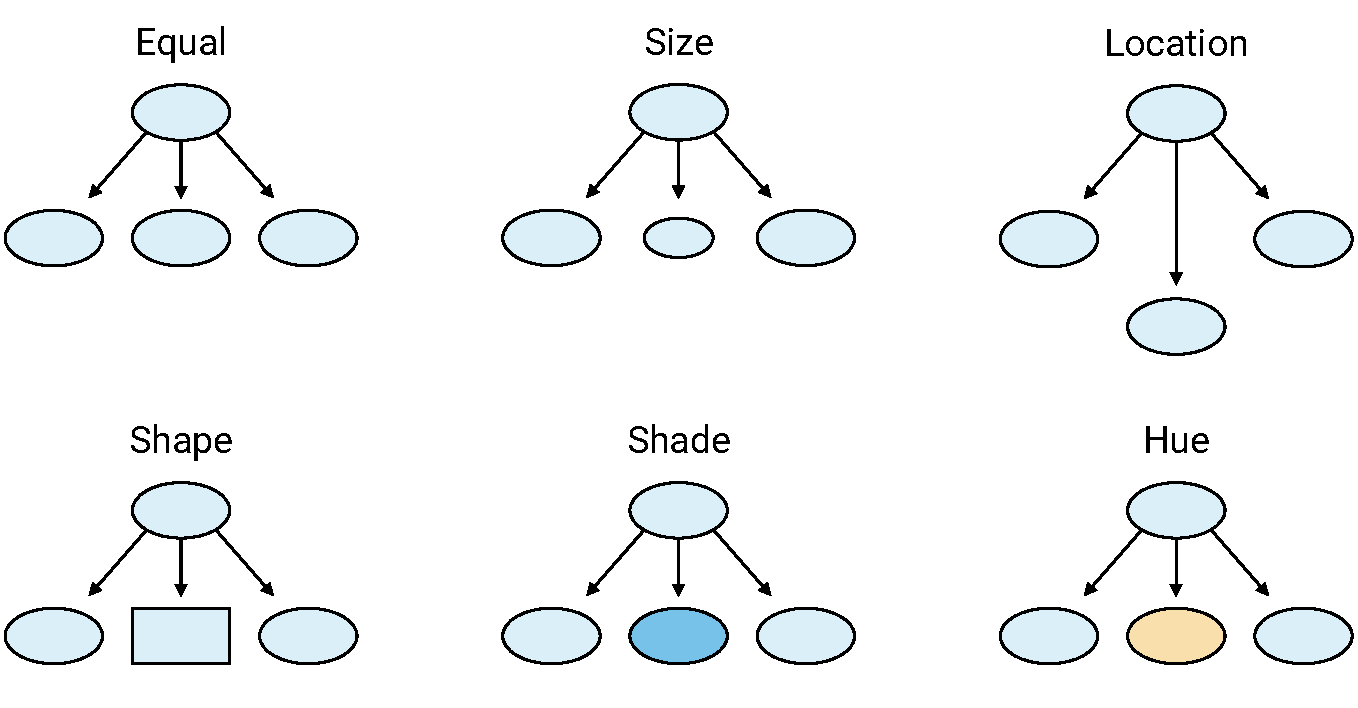
\includegraphics[width=1\textwidth]{diagram-emphasis}
\sidecaption{\label{fig:emphasis} Deviations from the norm create emphasis \cite{Carter12}.}[-4\baselineskip]
\end{figure}

Do not choose the size of elements arbitrarily. Differences translate into dominance relationships. Larger elements usually appear to control the smaller ones (cf. Fig.~\ref{fig:dominance})

\begin{figure}[t]
\centering
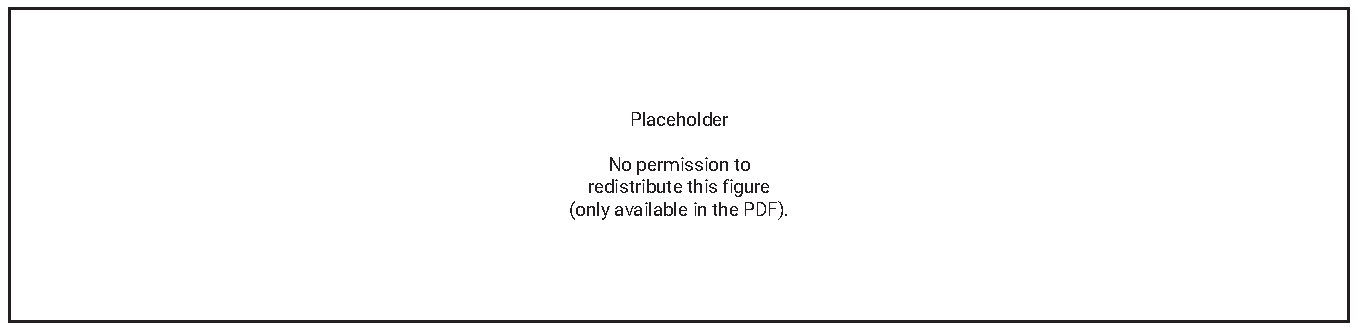
\includegraphics[width=1\textwidth]{diagram-dominance}
\sidecaption{\label{fig:dominance} Relative differences in size indicate dominance relationships \cite{Carter12}.}[-4\baselineskip]
\end{figure}


\subsection{Layout}

In the absence of strong emphasis, readers process diagrams similar to text (cf. Fig.~\ref{fig:direction}). In western cultures, readers will start in the top left corner and proceed horizontally in a zig-zag pattern. The general flow of information should be consistent with this expectation.

\begin{marginfigure}
\centering
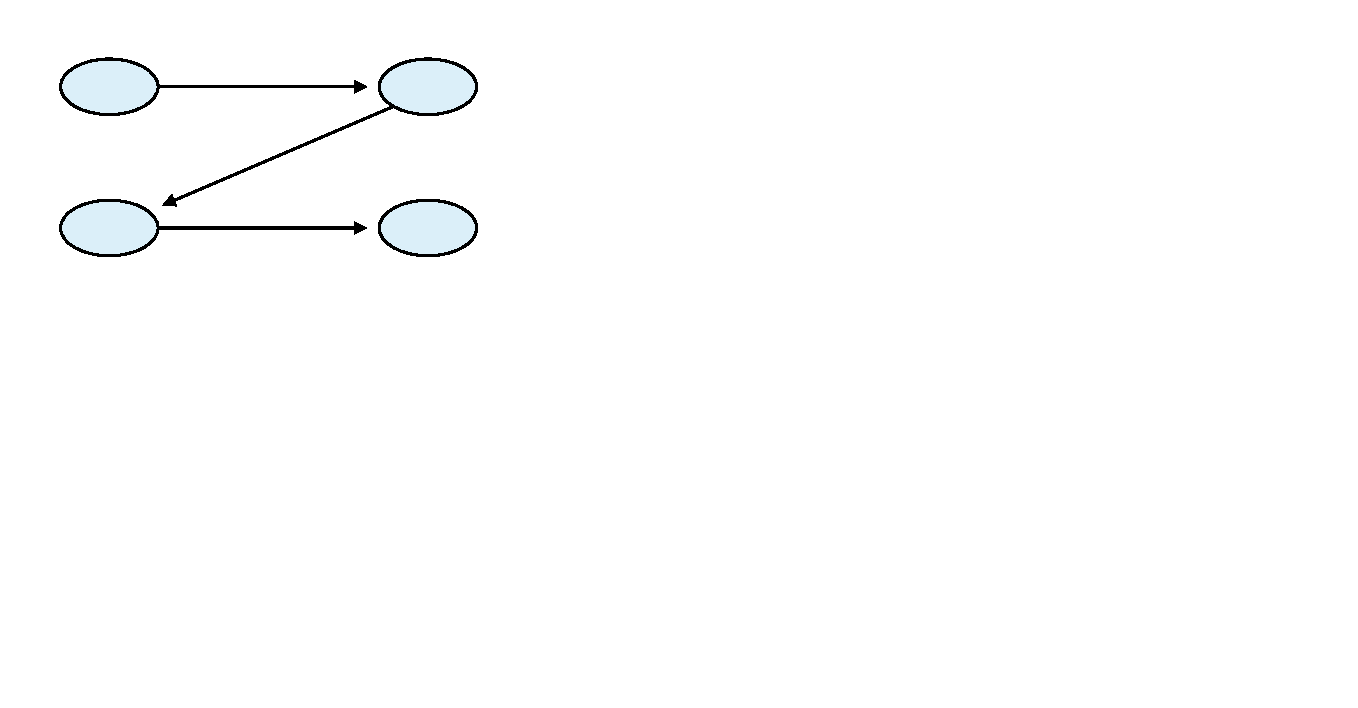
\includegraphics[width=1\textwidth]{diagram-direction}
\caption{\label{fig:direction} Respect the expected flow of information in western cultures \cite{Carter12}.}%[-1\baselineskip]
\end{marginfigure}


Ensure that all elements of a diagram are properly aligned. Alignment helps readers to grasp the overall structure. Proper alignment can also save you from creating additional outlines to depict (systems) boundaries – proximity and neat alignment can create strong cohesion by themselves (closure).

Make conscious decisions about distances and dimensions (proximity, repetition). You \emph{can} use a \emph{grid} to enforce consistent distances. Note, however, that snapping every element to the grid lines, may still cause mis-alignment in some cases.\sidenote{Consider a shape that is four grid lines high. Then, a horizontal line that leaves the box cannot be aligned in the middle.} Make use of the horizontal and vertical alignment tools that space out elements equally. An advanced technique is to create a dummy box shape to measure and compare dimensions yourself.

\subsection{Labels}

Many diagrams consist of shapes and lines, annotated with text labels.

A commonplace technique is to use bold print to express some property of an element. For instance, the labels of all shapes that correspond to systems are printed in bold to differentiate these shapes from the ones that correspond to exchanged  messages. In general, we recommend to avoid this practice. Reserve bold print for emphasizing \emph{one particular element} in a diagram. Use another visual style to signify differences, such as shading, colors, or shape form. Also consider the option of giving an element no surrounding shape at all, for instance, if the notion of its \emph{boundary} is not relevant.

In any case, the labels should be as close as possible to the shapes (proximity) and exactly aligned. Whenever possible, consider moving the labels into the shapes (Fig.~\ref{labelsinside}). Inside labels reduce visual clutter and make it easier to create a well-balanced diagram that has no ragged edges.

\begin{figure}[t]
\centering
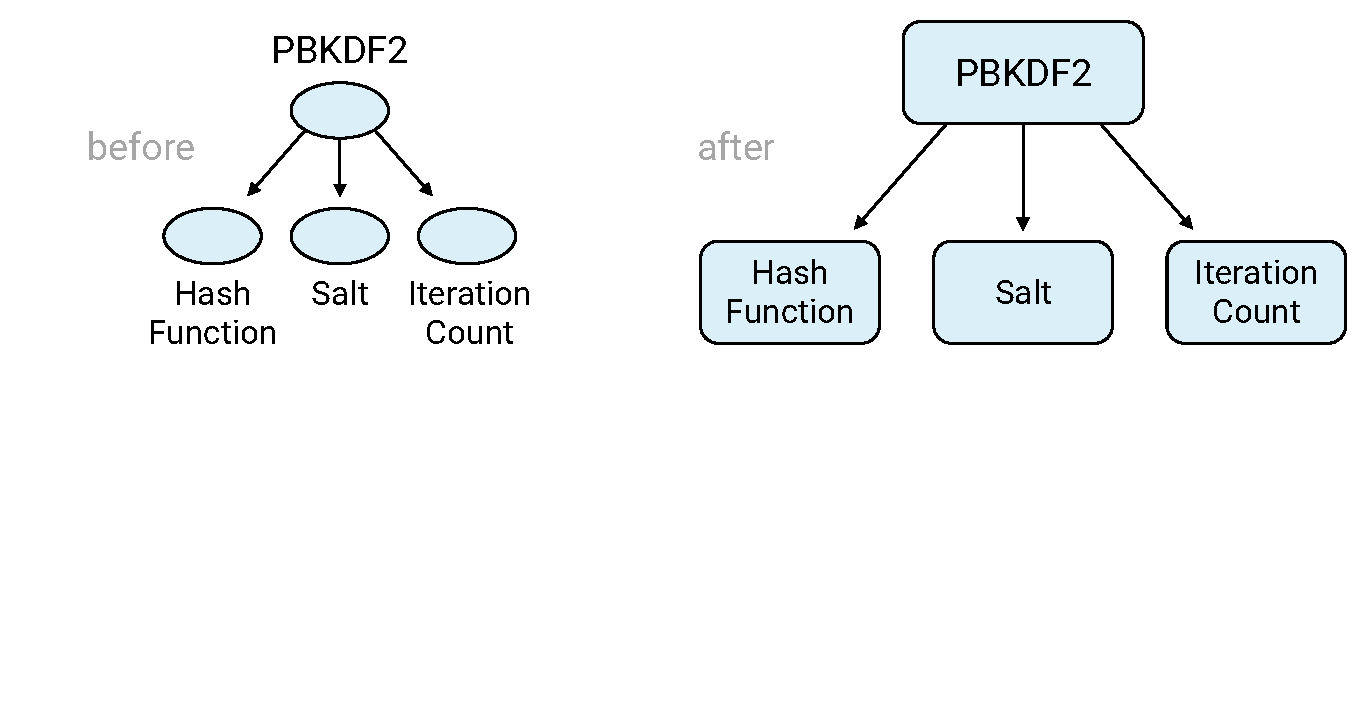
\includegraphics[width=1\textwidth]{diagram-labelsinside}
\sidecaption{\label{fig:dominance} Moving the labels inside objects reduces clutter. Note how the left-hand-side figure is centered in the left part of the figure to keep the figure balanced \cite{Carter12}.}[-6\baselineskip]
\end{figure}

\begin{marginfigure}
\centering
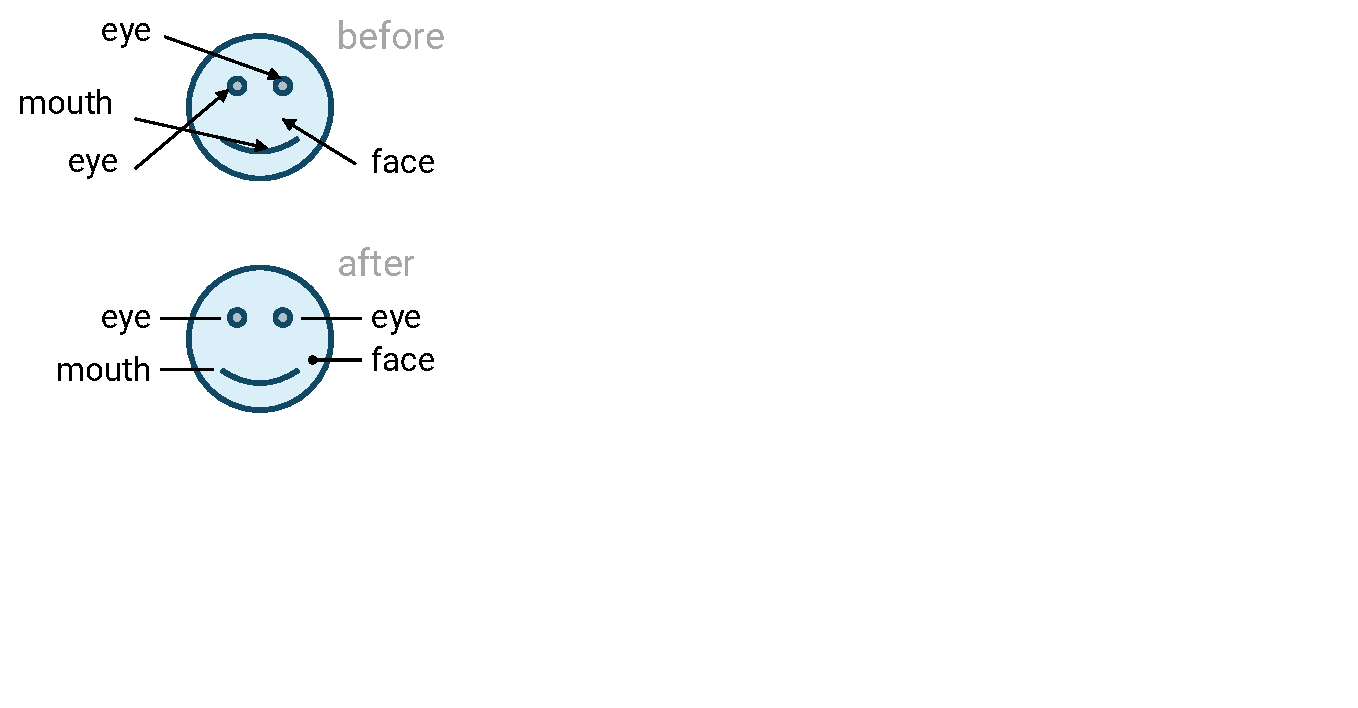
\includegraphics[width=1\textwidth]{diagram-labelsoutside}
\caption{\label{fig:labelsoutside} Outside labels should not distract the reader \cite{Carter12}.}%[-1\baselineskip]
\end{marginfigure}

Figure~\ref{fig:labelsoutside} illustrates key principles when labels are outside of a shape. First of all, keep the lines as short as possible (proximity). Consider removing the arrowheads from the lines that point into an object to avoid confusion with other arrows in the diagram. Also, avoid crossing lines. Align labels on the left-hand side of an object flush right and vice versa. Aim for consistency by making the lines parallel. Keep adequate amounts of surrounding whitespace.


\subsection{Variations}

\begin{figure*}[t]
\centering
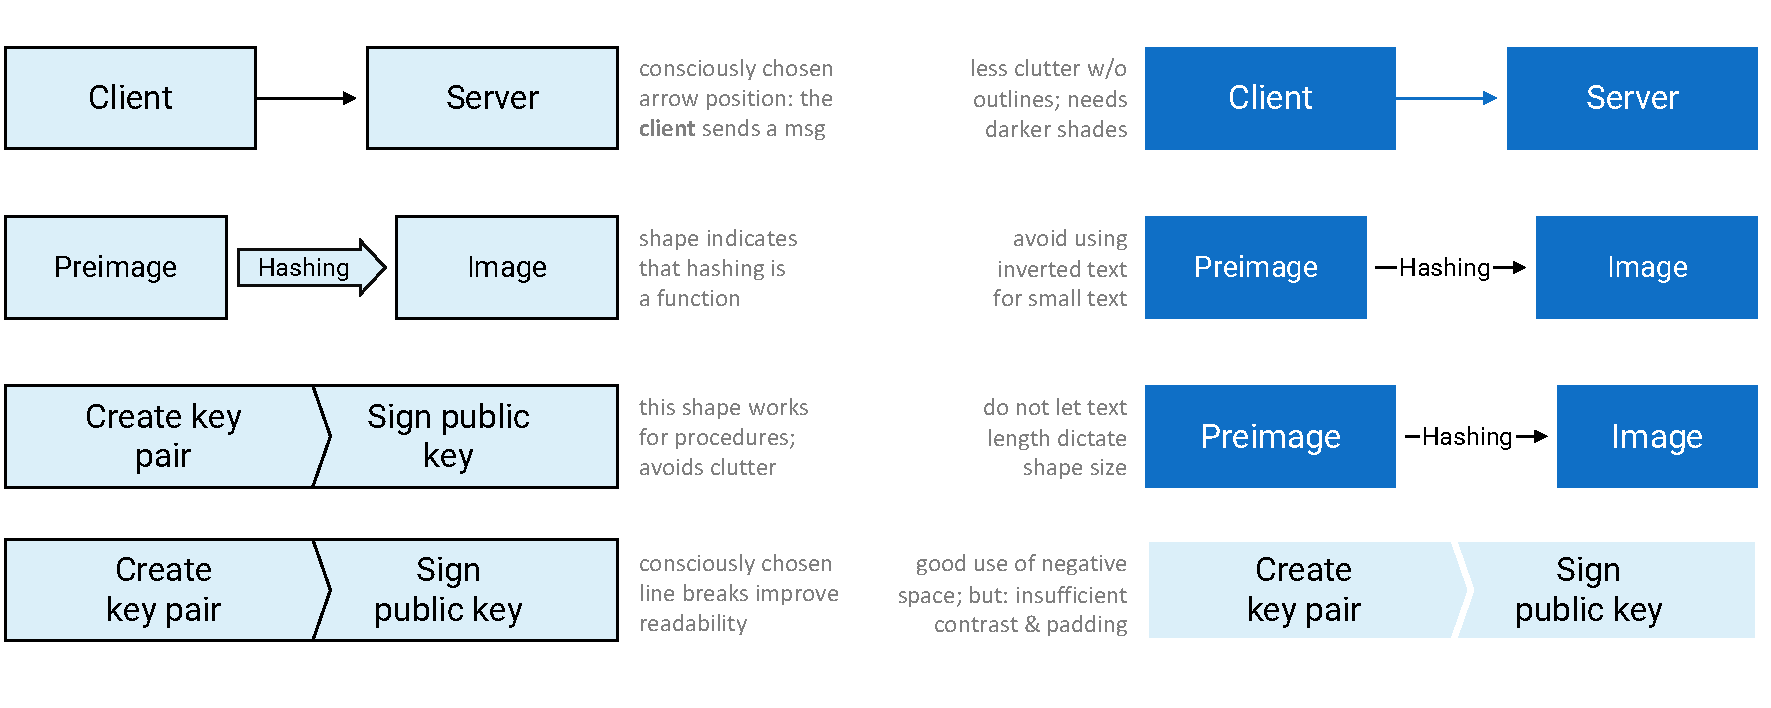
\includegraphics[width=1\widefigurewidth]{diagram-variations}
\sidecaption{\label{fig:diagvariations} Eight variations resulting from combining different outline, shade, and arrow styles.}[-1\baselineskip]
\end{figure*}

Common drawing tools provide a large number of shapes. What is missing, however, is guidance on how to combine them reasonably. Figure~\ref{fig:diagvariations} displays eight combinations.\sidenote{The advice in the following paragraphs has been compiled from \url{https://www.slideshare.net/otikik/how-to-make-awesome-diagrams-for-your-slides/19-Size_doesnt_mean_long_name}}

The first variation in the left-hand column shows a style useful for depicting information exchange between systems, such as servers and clients. The second variation uses an arrow shape. This emphasizes that the arrow corresponds to an activity itself. The third and fourth examples in the left-hand column depict two steps from a process without too much visual clutter. We prefer the latter one because the text wraps at sensible points.

The right-hand column shows variations without outlines. At first glance, this sounds like a good  idea: after all, it avoids visual clutter (the outlines). Note, however, that shapes without outlines need more saturated and darker color to differentiate them from the background.  If the number of shapes in a diagram is large, this approach can actually make it more difficult to read the diagram because all shapes appear to be emphasized at the same time.

If you use dark-colored shapes, you should avoid having white text on dark background for small font sizes. As shown in the second variation on the right-hand side of Fig.~\ref{fig:diagvariations}, you will have to make changes to some shapes.

In any case, you should choose the sizes of shapes consciously. Represent objects with identical properties with shapes of the same size. If the labels do not fit into the shapes, you can either reduce the font size, put the labels next to the box, or increase the size of all shapes (by rearranging the diagram).

Finally, consider the option of using negative space, as shown in the bottom-right corner of the Fig.~\ref{fig:diagvariations}.Again, this can be a useful means to avoid visual clutter. However, if you just increase the stroke width (as was done for the example figure), the (vertical) padding in the shape will become too narrow. Moreover, you cannot easily align such shapes with other shapes with thinner strokes.

\section{Figures}

















